\chapter{映像伝送システム}
\label{chap:video-transmission}

本章では、映像伝送システムを構成する技術要素の仕組みについて解説する。
% それぞれ、○○について述べる

\section{ビデオカメラ}
\label{sec:camera}


\section{ディスプレイ}
\label{sec:display}


\section{インターレース}
\label{sec:interlace}


\section{色空間と色深度}
\label{sec:colorspace}

一般的に液晶ディスプレイでは、1ピクセルを赤、緑、青、すなわちRGBの3つの色信号で表現する。
多くのPCやゲーム機の出力ではRGBの色空間が使われ、RGBそれぞれ8bit、1ピクセルあたり24bitで表現する。
1ピクセルあたりを表現するビット数を色深度といい、色解像度、色分解能とも言われる。
24bitの色深度では、16,777,216色を表現することができる。

一方、ビデオカメラでは、輝度信号Yと、2つの色差信号を使って表現される色空間であるYUVが使われるが多い。[要出典]
この方式の特徴は、「人間の目は明るさの変化には敏感だが、色の変化には鈍感である」という性質に基づいて、色度信号の情報量を減らすことができるという点にある。

\begin{figure}[htbp]
    \begin{center}
        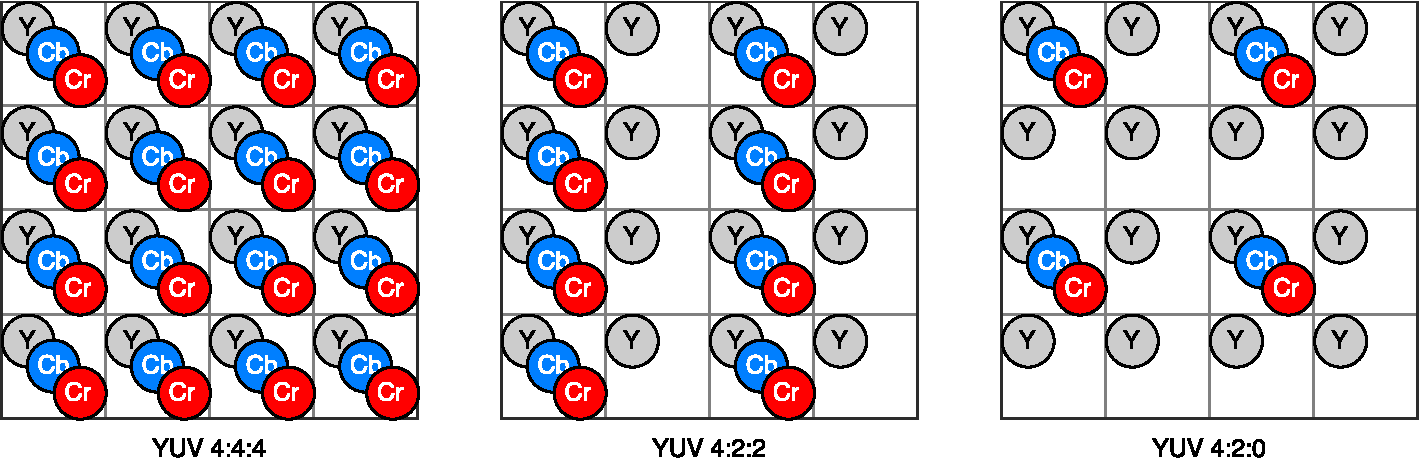
\includegraphics[bb=0 0 681 222,width=14cm]{img/yuv-pixel-structure.pdf}
    \end{center}
    \caption{YUVのピクセルあたりの色情報の構造}
    \label{fig:yuv-pixel-structure}
\end{figure}

% YUVのピクセルあたりの色情報の構造を、図\ref{fig:yuv-pixel-structure}に示す。

YUV 4:4:4では、輝度信号、色差信号共に1ピクセル毎である。
YUV 4:2:2では、輝度信号は1ピクセル毎、色差信号は2ピクセル毎であり、同じ色深度のYUV 4:4:4と比べ、帯域はおよそ2/3となる。
YUV 4:2:0では、輝度信号は1ピクセル毎、色差信号は4ピクセル毎であり、同じ色深度のYUV 4:2:2と比べ、帯域はおよそ3/4となり、同じ色深度のYUV 4:4:4と比べ、帯域はおよそ1/2となる。

% 図\ref{fig:yuv-pixel-structure}のCb、Crの、どこのピクセルの色情報を扱うかは、伝送方式の規格によって異なる。

\section{帯域}
\label{sec:bandwidth}
% この部分はあとで何処かに持っていく予定

帯域は解像度の他にも、インターレース、色空間、色深度により変化する。

表は次のように出力される。(表\ref{tb:video-bandwidth})
色深度は8bitとする。

また、1920x1080、
1920x1080p/60 2200x1125 148.5 SMPTE 274M

1Channel = 2200 * 1125 * 3 * 8 * 60 * 1.25/3

\begin{table}[htbp]
  \caption{解像度、フレームレート、色空間による帯域の変化}
  \label{tb:video-bandwidth}
  \begin{center}
  \begin{tabular}{c|c|c|c|c|c}
    \hline
    解像度     & フレームレート & 色空間  & ピクセルクロック & 帯域     & 同期区間を含んだ帯域 \\\hline\hline
    3840x2160 & 60p          & RGB    & 1.485MHz      & XX Gbps & YY Gbps           \\\hline
    3840x2160 & 60p          & YUV422 & 1.485MHz      & XX Gbps & YY Gbps           \\\hline
    3840x2160 & 60p          & YUV420 & 1.485MHz      & XX Gbps & YY Gbps           \\\hline
    3840x2160 & 30p          & RGB    & 1.485MHz      & XX Gbps & YY Gbps           \\\hline
    3840x2160 & 30p          & YUV422 & 1.485MHz      & XX Gbps & YY Gbps           \\\hline
    1920x1080 & 60p          & RGB    & 1.485MHz      & XX Gbps & YY Gbps           \\\hline
    1920x1080 & 60p          & YUV422 & 1.485MHz      & XX Gbps & YY Gbps           \\\hline
    1920x1080 & 60i          & RGB    & 1.485MHz      & XX Gbps & YY Gbps           \\\hline
    1920x1080 & 60i          & YUV422 & 1.485MHz      & XX Gbps & YY Gbps           \\\hline
  \end{tabular}\end{center}
\end{table}

\section{インターフェース}
\label{sec:interface}

\subsection{VGA}


\subsection{DVI}
Digital Visual Interface
Transition Minimized Differential Signaling、TMDS
VESA(Video Electronics Standards Association)によって標準化された デジタル映像信号の伝送方式。
であり、
赤、緑、青、クロックの4つのツイストペアケーブルで構成される。

\subsection{HDMI}
1.4 / 2.0

HDMI 2.0からは、YCbCr 4:2:0方式によるピクセルエンコーディングの規格が追加され、1/2のデータレートで転送することが可能となった。

\begin{table}[htbp]
  \caption{HDMI 1.4と2.0での4K(3840x2160)映像の対応状況}
  \label{tb:video-bandwidth}
  \begin{center}
  \begin{tabular}{c|c|c|c}
    \hline
      フレームレート & ピクセルあたりの色深度 & HDMI 1.4 & HDMI 2.0\\\hline\hline
    \multirow{4}{*}{30Hz} &
        24bit & 対応   & 対応 \\\cline{2-4}
      & 30bit & 対応   & 対応 \\\cline{2-4}
      & 36bit & 対応   & 対応 \\\cline{2-4}
      & 48bit & 非対応 & 対応 \\\hline
    \multirow{4}{*}{60Hz} &
        24bit & 非対応 & 対応  \\\cline{2-4}
      & 30bit & 非対応 & 対応  \\\cline{2-4}
      & 36bit & 非対応 & 対応  \\\cline{2-4}
      & 48bit & 非対応 & 非対応 \\\hline
  \end{tabular}\end{center}
\end{table}

HDMI 1.4\cite{hdmi-spec-1-4}では、RGB、YCbCr 4:4:4、YCbCr 4:2:2の色空間がサポートされており、HDMI 2.0\cite{hdmi-spec-2-0}では、新たに4K解像度向けのYCbCr 4:2:0がサポートされた。

また、YCbCr方式

すなわち、HDMIでは色空間のYCbCr 4:4:4、YCbCr 4:2:2のどちらであっても帯域には影響しない。

% すなわち、\ref{sec:colorspace}章では、色深度
\begin{figure}[htbp]
    \begin{center}
        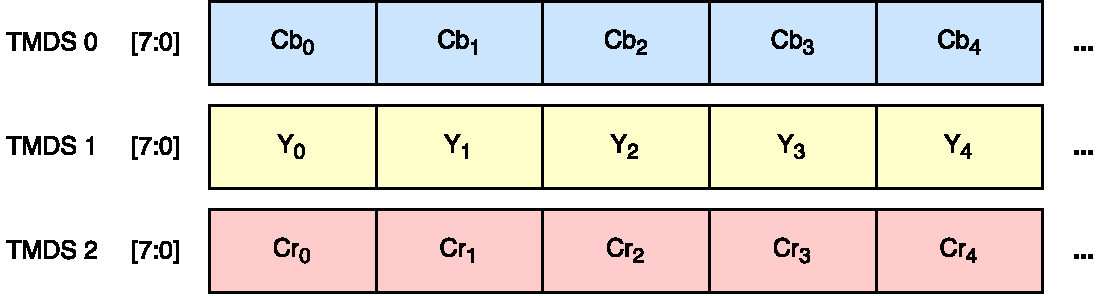
\includegraphics[bb=0 0 531 141,width=13.926cm]{img/hdmi-spec-yuv-444.pdf}
    \end{center}
    \caption{Video Stream to Ethernet Packet Subsystem Diagram}
    \label{fig:hdmi-spec-yuv-444}
\end{figure}

\begin{figure}[htbp]
    \begin{center}
        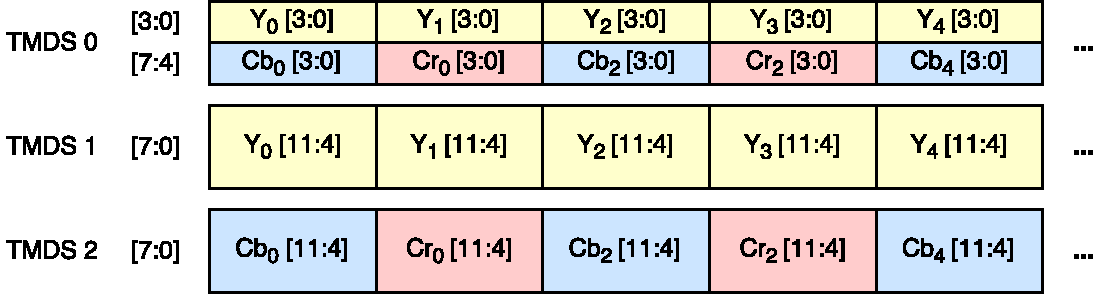
\includegraphics[bb=0 0 531 141,width=13.926cm]{img/hdmi-spec-yuv-422.pdf}
    \end{center}
    \caption{Video Stream to Ethernet Packet Subsystem Diagram}
    \label{fig:hdmi-spec-yuv-422}
\end{figure}

\begin{figure}[htbp]
    \begin{center}
        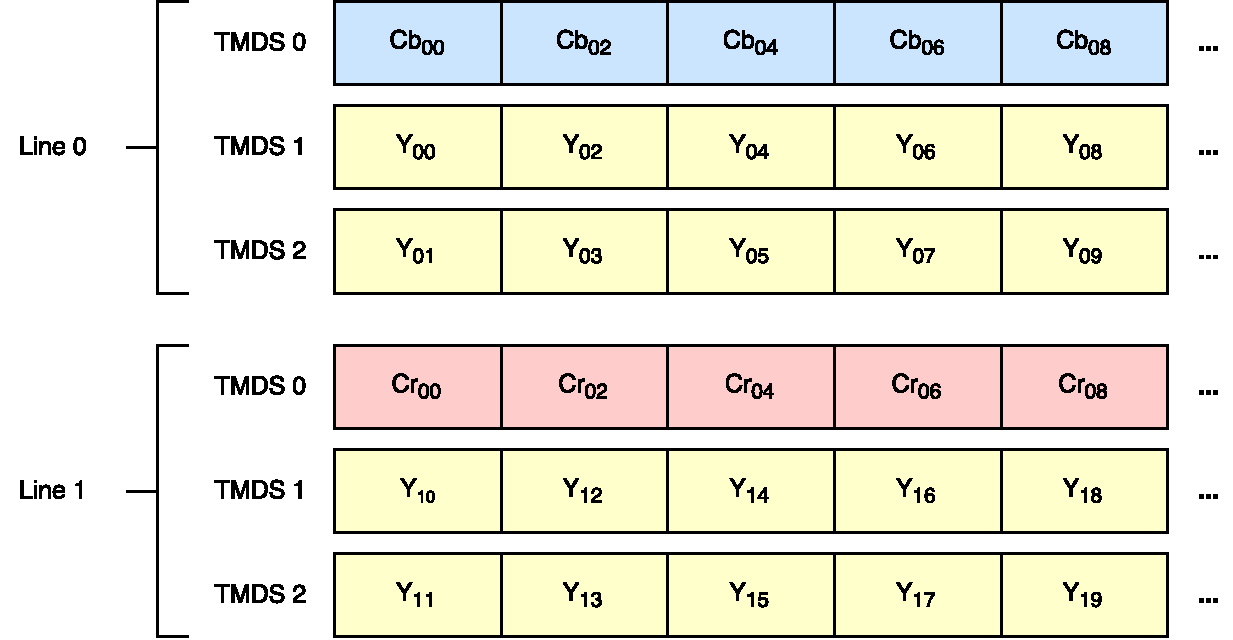
\includegraphics[bb=0 0 591 306,width=15.5cm]{img/hdmi-spec-yuv-420.pdf}
    \end{center}
    \caption{Video Stream to Ethernet Packet Subsystem Diagram}
    \label{fig:hdmi-spec-yuv-420}
\end{figure}

\subsection{SDI}

同軸ケーブルを用いた映像伝送方式
ロック

\section{伝送手法}

\section{まとめ}
